\documentclass[a4paper, 11pt]{article}
\usepackage{graphicx}
\usepackage{wrapfig}

\begin{document}
\title{EE568 Project 2: Motor Winding Design \& Analysis}
\author{Baris Kuseyri}
\date{\today}
\maketitle

\pagenumbering{arabic}
\tableofcontents
\newpage


\section{Integral-Slot Winding Design}
\subsection{Winding Diagram}

\begin{wrapfigure}{r}{0.5\textwidth}
	\vspace{-20pt}
	\begin{center}
		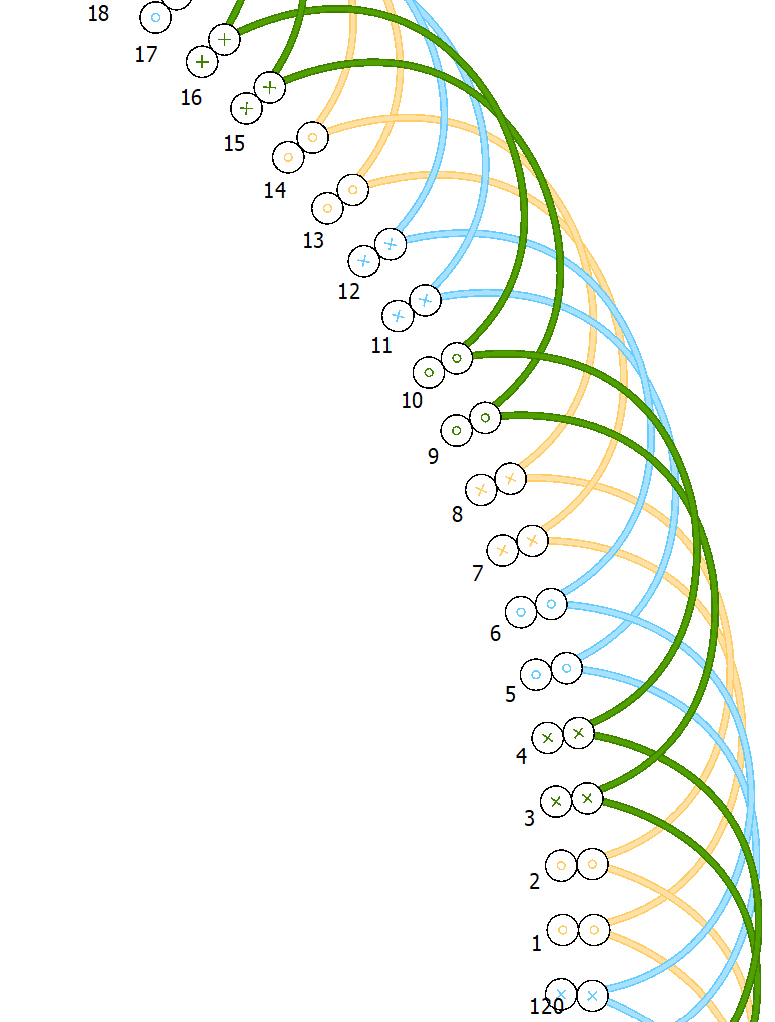
\includegraphics[width=0.3\textwidth]{Q1_windingDiagram_1pp_dolomites.png}
	\end{center}
	\vspace{-20pt}
	\caption{Winding Diagram: 1 pole-pair}
	\vspace{-10pt}
\end{wrapfigure}

\begin{wrapfigure}{r}{0.5\textwidth}
	\vspace{-20pt}
	\begin{center}
		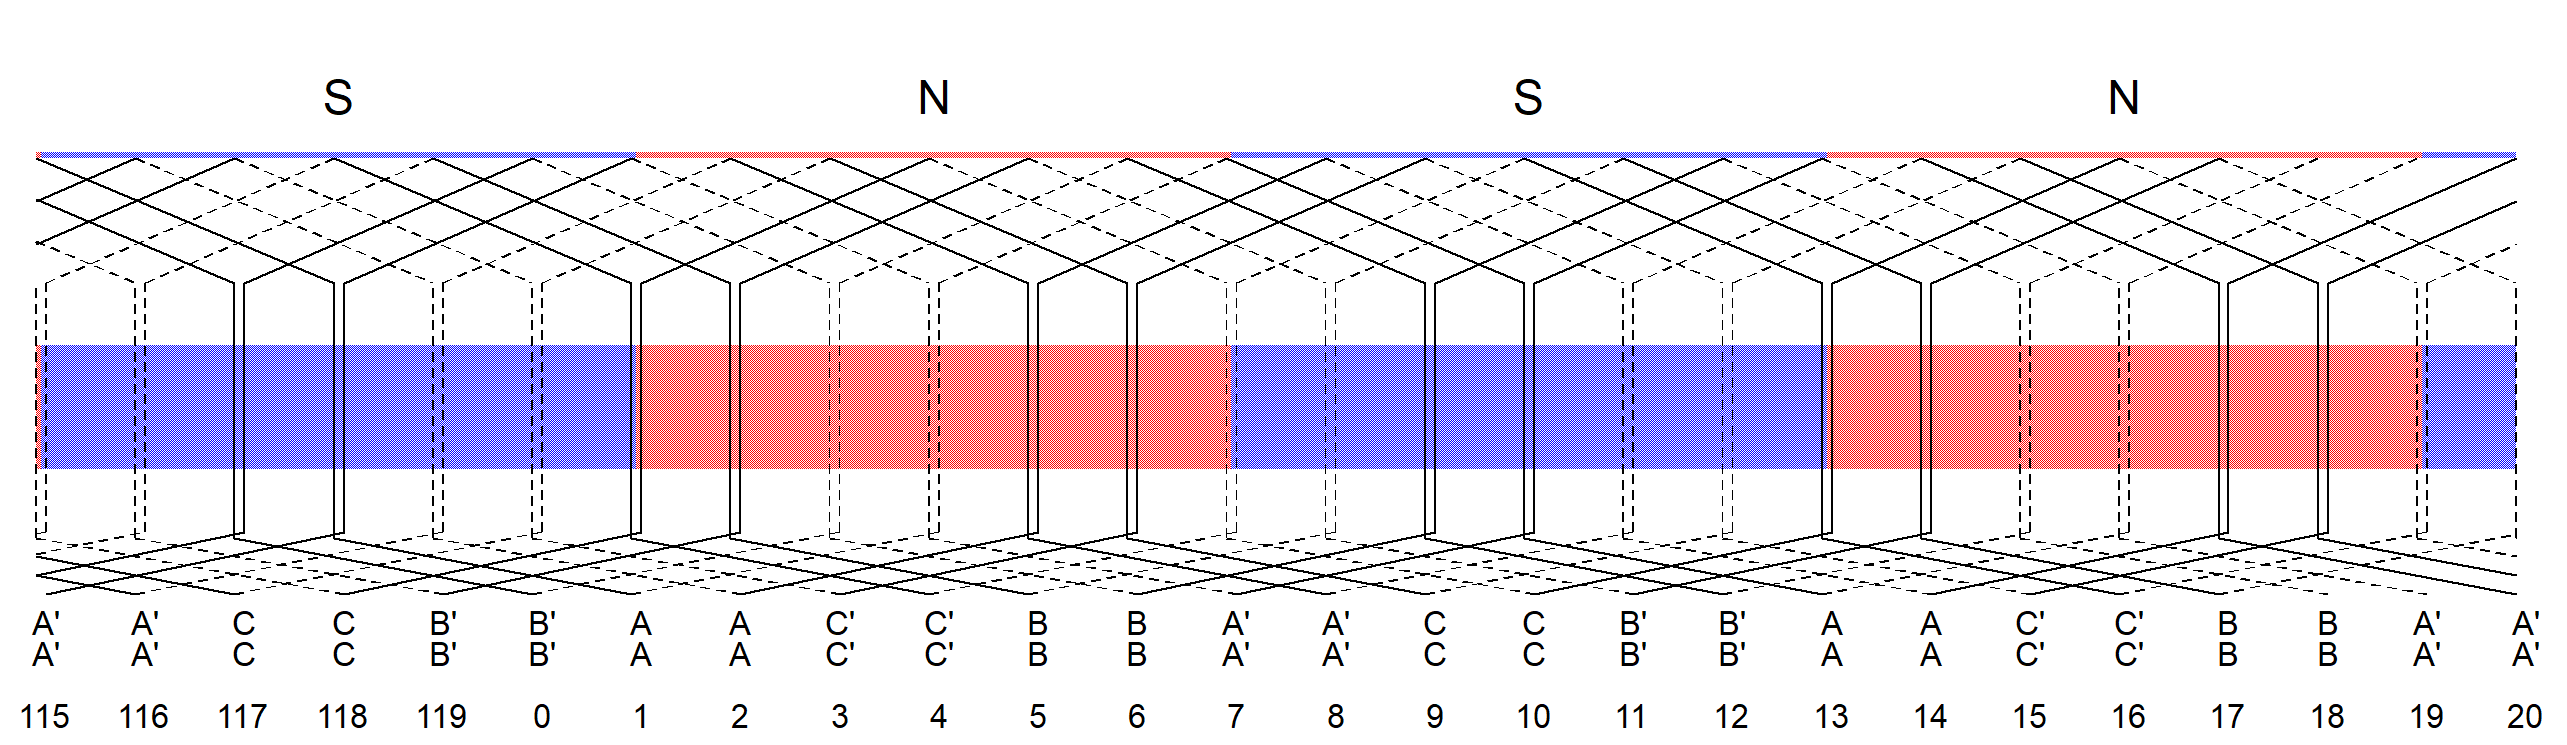
\includegraphics[width=1.0\textwidth]{Q1_windingDiagram_1pp.png}
	\end{center}
	\vspace{-20pt}
	\caption{Winding Diagram: 1 pole pair}
	\vspace{-10pt}
\end{wrapfigure}

\subsection{Distribution, Pitch and Winding Factors}

\section{Fractional-Slot Winding Design}
\subsection{27-slot/22-pole EM}
\subsubsection{Phase Angle of Induced Voltage in each Slot}
\subsubsection{Phasor Diagram}
\subsubsection{Distribution, Pitch and Winding Factors}
\subsubsection{Phase Angle of Induced Voltage in each Slot}
\subsection{24-slot/22-pole EM}

\section{2-D FEA Modelling}

\end{document}